\documentclass{article}

% Cabecera del documento
% ======================================================================

% Paquetes extras
\usepackage[square, numbers, sort]{natbib}
% \usepackage{cite}
\usepackage{graphicx}
\usepackage{subcaption}
\usepackage[utf8]{inputenc}
\usepackage{amsmath,amssymb,amsfonts}
\usepackage{algorithmic}
\usepackage{textcomp}
\usepackage{float}
\usepackage{mathtools}
\usepackage[spanish]{babel}
\usepackage[paper=a4paper,margin=2.75cm]{geometry}
\usepackage{booktabs} % for tables
\usepackage[colorlinks = true,
            linkcolor = blue,
            urlcolor  = blue,
            citecolor = orange,
            anchorcolor = blue]{hyperref} % for hyperlinks
\usepackage{xcolor} % text colors

% Directorio con imagenes
\graphicspath{{./figs/}}

% Cabecera del documento
% ======================================================================

% Titulo
\title{Diseño de controlador para sistema de Steering-by-Wire}

% Autores
\author{Rodrigo Aleo - 12106\\ aleorodrigof@gmail.com \\ \\ Control y Sistemas, Facultad de Ingeniería, \\ Universidad Nacional de Cuyo, \\ Mendoza, Argentina}

% Fecha
\date{Julio de 2025, versión v001}

% Cuerpo del documento
% ======================================================================
\begin{document}

% Comandos definidos por el autor
\renewcommand{\tablename}{Tabla}
% \renewcommand{\color{blue}{#1}}{\azul}

% Crear cabecera
\maketitle

% Resumen
% ======================================================================
\begin{abstract}
    El presente documento presenta los contenidos mínimos que debe tener el proyecto final de la cátedra de Control y Sistemas de la Universidad Nacional de Cuyo. Además, se aclara el estilo de redacción que debe tener el informe del proyecto final y se facilitan algunos recursos para la edición de documentos en \LaTeX.  
\end{abstract}

% Secciones
% ======================================================================
\section{Introducción}
\label{sec:intro}

% En la sección \ref{sec:intro}... 

En un sistema de direccionamiento de un automóvil convencional, el conductor induce en el volante una rotación que es transmitida mediante una conexión mecánica hacia las ruedas del automóvil. Una simplificación de dicho mecanismo puede observarse en la figura \ref{fig:dir_convencional}.

\begin{figure}[H]
    \centering
    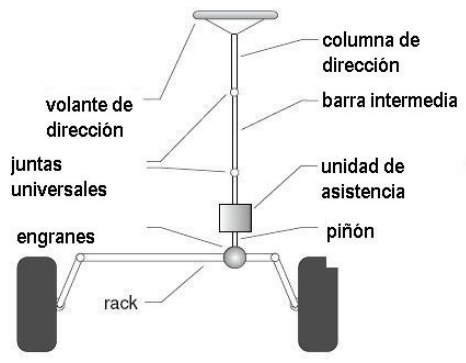
\includegraphics[width=0.5\linewidth]{figs/Sistema de direccionamiento convencional.png}
    \caption{Sistema de direccionamiento convencional (simplificado)}
    \label{fig:dir_convencional}
\end{figure}

El sistema de \textit{Dirección por Cable} (\textit{Steering-by-wire} o \textit{SbW}) elimina la columna de dirección convencional que conecta el volante con el mecanismo de rotación de las ruedas, y la reemplaza por una interfaz completamente electrónica, como se ilustra en la figura \ref{fig:dir_SbW}. Un sensor de posición angular ubicado en el volante envía la señal a un controlador, el cual comanda un actuador electromecánico responsable del giro de las ruedas. Adicionalmente, puede integrarse un motor de retroalimentación en el volante que reproduzca las fuerzas generadas en las ruedas, con el objetivo de conservar la sensación de contacto con el terreno.

Este enfoque constituye una innovación relevante en el ámbito automotriz, y presenta múltiples ventajas:

\begin{itemize}
    \item Reducción del peso y la complejidad del sistema, al eliminar componentes mecánicos.
    \item Mejora en la seguridad, al permitir intervenciones del sistema ante condiciones adversas, como pérdida de adherencia.
    \item Posibilidad de modificar la relación entre el ángulo de giro del volante y el ángulo de las ruedas en función de la velocidad y otras variables, optimizando así la dinámica del vehiculo.
    \item Mayor flexibilidad en el diseño del habitáculo, al no requerir una conexión física entre el volante y el tren delantero.
    \item Disminución del peso general del automóvil a remover elementos mecánicos.
\end{itemize}

\begin{figure}[H]
    \centering
    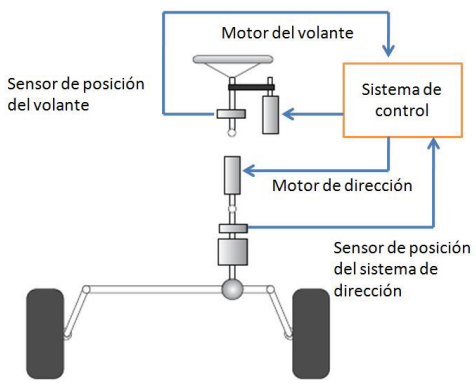
\includegraphics[width=0.6\linewidth]{figs/SbW Modelo Sencillo.png}
    \caption{Modelo simplificado de SbW}
    \label{fig:dir_SbW}
\end{figure}
% ======================================================================
\section{Desarrollo}
\subsection{Modelado de la planta}
El sistema de direccionamiento de las ruedas consiste en un motor de corriente continua que acciona un sistema piñón-cremallera. La cremallera, al moverse lateralmente, acciona una rótula que permite la rotación de las ruedas. En la figura \ref{fig:esquema_planta} puede verse una representación del sistema:
\begin{figure}[H]
    \centering
    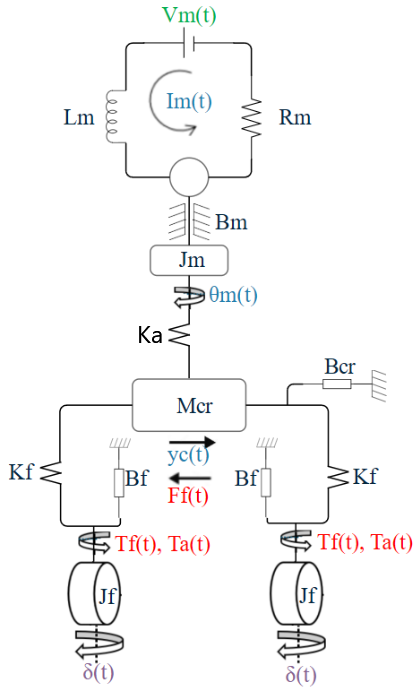
\includegraphics[width=0.5\linewidth]{figs/Esquema_planta.png}
    \caption{Esquema simplificado del sistema de dirección del tren delantero.}
    \label{fig:esquema_planta}
\end{figure}

La ecuación eléctrica del motor de CC es obtenida usando reglas de Kirchoff:
\begin{equation}
L_m \cdot \frac{di_m}{dt} = -R_m \cdot i_m(t) - K_e \cdot \omega_m(t) + V_m(t)
\label{ec_electrica}
\end{equation}

Donde:
\begin{itemize}
    \item $V_m(t)$: Tensión aplicada al motor ($\mathrm{V}$). Es la entrada del sistema eléctrico.
    \item $L_m$: Inductancia de la bobina del motor ($\mathrm{H}$).
    \item $R_m$: Resistencia de la bobina del motor ($\mathrm{\Omega}$).
    \item $i_m(t)$: Corriente instantánea que circula por la fase del motor ($\mathrm{A}$).
    \item $K_e$: Constante de fuerza contraelectromotriz ($\mathrm{V \cdot s/rad}$).
    \item $\omega_m(t)$: Velocidad angular del rotor ($\mathrm{rad/s}$). 
\end{itemize}

Para el modelado matemático de los mecanismos se utilizan leyes de Newton. Para el eje motor:
\begin{equation}
J_m \cdot \frac{d\omega(t)}{dt} = T_m(t) - B_m \cdot \omega_m(t) - K_{a} \left[ \theta_m(t) - \frac{y_c(t)}{r_p} \right]
\label{ec_motor}
\end{equation}

Donde:
\begin{itemize}
    \item $\theta_m(t)$: Posición angular del rotor ($\mathrm{rad}$). Relacionada con $\omega_m$ mediante: $\frac{d\theta_m(t)}{dt} = \omega(t)$.
    \item $J_m$: Momento de inercia del rotor ($\mathrm{kg \cdot m^2}$).
    \item $T_m(t)$: Par generado por el motor ($\mathrm{N \cdot m}$). Se considera proporcional a la corriente mediante la constante de par motor $K_t$ ($\mathrm{\frac{N \cdot m}{A}}$). Luego: $T_m(t) = K_t \cdot i_m(t)$.
    \item $B_m$: Coeficiente de fricción viscosa del eje ($\mathrm{\frac{N \cdot m \cdot s}{rad}}$). Modela las pérdidas mecánicas por fricción.
    \item $K_{a}$: Constante de rigidez del acoplamiento elástico ($\mathrm{\frac{N \cdot m}{rad}}$). Representa la holgura entre el piñón y la cremallera. Si este valor tendiera a infinito, se estaría considerando un acoplamiento perfecto entre los engranajes. Se utiliza este componente elástico para representar la falta de transmisión directa entre el motor y la cremallera.
    \item $y_c(t)$: Desplazamiento lineal de la cremallera ($\mathrm{m}$).
    \item $r_p$: Radio efectivo del piñón ($\mathrm{m}$). Para ángulos pequeños, convierte la rotación del piñón $\theta_p$ a un desplazamiento lineal de la cremallera mediante $\theta_p \cdot r_p = y_c$.
\end{itemize}

La ecuación dinámica de la cremallera es:
\begin{equation}
M_{cr} \cdot \frac{dv_c(t)}{dt} = -\frac{2 K_f}{r_l} \left[ \frac{y_c(t)}{r_l} - \delta(t) \right] - F_f(t) - B_{cr} \cdot v_c(t) + \frac{K_a}{r_p} \left[ \theta_m(t) - \frac{y_c(t)}{r_p} \right]
\label{ec_cremallera}
\end{equation}

Donde:
\begin{itemize}
    \item $M_{cr}$: Masa de la cremallera ($\mathrm{kg}$).
    \item $v_c(t)$: Velocidad lineal de la cremallera ($\mathrm{\frac{m}{s}}$). Se relaciona con $y_c$ mediante: $\frac{dy_c(t)}{dt}=v_c(t)$
    \item $K_f$: Rigidez del enlace entre la cremallera y la rueda ($\mathrm{\frac{N \cdot m}{rad}}$). Notar que el término figura duplicado en la ecuación debido a la contribución de cada neumático.
   \item $\delta(t)$: Ángulo de giro del neumático medido desde la posición de avance rectilíneo del vehículo ($\mathrm{rad}$).
    \item $r_l$: distancia horizontal entre el eje del pivote y el centro de la rueda($m$). Relaciona desplazamientos lineales de la cremallera, con rotaciones en la rueda mediante $\delta(t) \cdot r_l =  y_c(t)$, para ángulos pequeños de $\delta(t)$.
    \item $F_f(t)$: Fuerza de fricción estática en la cremallera ($\mathrm{N}$).
    \item $B_{cr}$: Coeficiente de fricción viscosa de la cremallera ($\mathrm{\frac{N \cdot s}{m}}$).
\end{itemize}

Finalmente, la ecuación dinámica de cada rueda está dada por:
\begin{equation}
J_f \cdot \frac{d\psi_f(t)}{dt} = -K_f \left[ \delta(t) - \frac{y_c(t)}{r_l} \right] - B_f \cdot \omega_f(t) - T_f(t) - T_a(t)
\label{ec_rueda}
\end{equation}

Donde:
\begin{itemize}
    \item $J_f$: Momento de inercia de la rueda ($\mathrm{kg \cdot m^2}$).
    \item $\psi_f(t)$: Velocidad angular de giro del neumático en el plano de dirección ($\mathrm{rad/s}$). Relacionado con $\delta(t)$ mediante: $\frac{d\delta_f(t)}{dt} = \psi(t)$
    \item $T_f(t)$: Torque de fricción estática del mecanismo de dirección ($\mathrm{N \cdot m}$).
    \item $T_a(t)$: Torque de autoalineamiento generado por las deformaciones del neumático al rotar mientras el auto está en velocidad no nula($\mathrm{N \cdot m}$).
\end{itemize}

En la tabla \ref{tab:parametros_modelo} pueden verse un resumen de todos los parámetros que intervienen en el sistema, junto a los valores que se les ha sido asignados.

\begin{table}[H]
\small
\centering
\caption{Parámetros del modelo de dirección por cable}
\label{tab:parametros_modelo}
\begin{tabular}{l c c}
\toprule
\textbf{Símbolo} & \textbf{Valor} & \textbf{Unidad} \\
\midrule
$L_m$     & $0.002$   & $\mathrm{H}$ \\
$R_m$     & $0.6$     & $\mathrm{\Omega}$ \\
$B_m$     & $1$       & $\mathrm{N \cdot m \cdot s / rad}$ \\
$J_m$     & $1.9$     & $\mathrm{kg \cdot m^2}$ \\
$K_e$     & $0.35$    & $\mathrm{V \cdot s / rad}$ \\
$K_t$     & $0.35$    & $\mathrm{N \cdot m / A}$ \\
\midrule
$K_a$     & $3500$    & $\mathrm{N \cdot m / rad}$ \\
\midrule
$B_{cr}$  & $1.032$   & $\mathrm{N \cdot s / m}$ \\
$M_{cr}$  & $2.0$     & $\mathrm{kg}$ \\
$r_l$     & $0.3$     & $\mathrm{m}$ \\
$r_p$     & $0.035$   & $\mathrm{m}$ \\
\midrule
$B_f$     & $30$      & $\mathrm{N \cdot m \cdot s / rad}$ \\
$K_f$     & $26000$   & $\mathrm{N \cdot m / rad}$ \\
$I_f$     & $0.270$   & $\mathrm{kg \cdot m^2}$ \\
\bottomrule
\end{tabular}
\end{table}



Teniendo en cuenta las ecuaciones \ref{ec_electrica}, \ref{ec_motor}, \ref{ec_cremallera} y \ref{ec_rueda}, puede armarse el siguiente sistema de ecuaciones:


\begin{equation}
\left\{
\begin{aligned}
\frac{di_m(t)}{dt} &= \frac{1}{L_m} \cdot  \left[-R_m \cdot i_m(t) - K_e \cdot \omega_m(t) + V_m(t) \right] \\
\frac{d\theta_m(t)}{dt} &= \omega(t) \\
\frac{d\omega_m(t)}{dt} &= \frac{1}{J_m} \cdot \left\{T_m(t) - B_m \cdot \omega_m(t) - K_{a} \left[ \theta_m(t) - \frac{y_c(t)}{r_p} \right] \right\} \\
\frac{dy_c(t)}{dt} &= v_c(t) \\
\frac{dv_c(t)}{dt} &= \frac{1}{M_{cr}} \cdot \left\{ -\frac{2 K_f}{r_l} \left[ \frac{y_c(t)}{r_l} - \delta(t) \right] - F_f(t) - B_{cr} \cdot v_c(t) + \frac{K_a}{r_p} \left[ \theta_m(t) - \frac{y_c(t)}{r_p} \right] \right\} \\
\frac{d\delta_f(t)}{dt} &= \psi(t) \\
\frac{d\psi_f(t)}{dt} &= \frac{1}{J_f} \cdot \left\{ -K_f \left[ \delta(t) - \frac{y_c(t)}{r_l} \right] - B_f \cdot \omega_f(t) - T_f(t) - T_a(t) \right\}
\end{aligned}
\right.
\label{sistema_completo}
\end{equation}

Debido a que el sistema es lineal, puede ser representado de forma matricial utilizando espacio de estados:

\begin{equation}
\left\{
\begin{aligned}
\dot{x}(t) &= A \cdot x(t) + B_c \cdot u(t) + B_d \cdot d(t) ;\quad x(0) = 0\\
y(t) &= C \cdot x(t)
\end{aligned}
\right.
\label{ec_SS}
\end{equation}

Las variables de estado quedan definidas en el vector $x(t)$, y se relacionan entre sí mediante la matriz dinámica del sistema $A$:
\begin{equation*}
x(t) =
\begin{bmatrix}
i_m(t) &
\theta_m(t) &
\omega_m(t) &
y_c(t) &
v_c(t) &
\delta(t) &
\psi(t)
\end{bmatrix}^T
\end{equation*}

\begin{equation}
A =
\begin{bmatrix}
-\frac{R_m}{L_m} & 0 & -\frac{K_e}{L_m} & 0 & 0 & 0 & 0 \\
0 & 0 & 1 & 0 & 0 & 0 & 0 & \\
\frac{K_t}{J_m} & -\frac{K_a}{J_m} & -\frac{B_m}{J_m} & \frac{K_a}{r_p\cdot J_m} & 0 & 0 & 0 \\
0 & 0 & 0 & 0 & 1 & 0 & 0 \\
0 & \frac{K_a}{r_p \cdot M_{cr}} & 0 & -\left(\frac{2\cdot K_f}{r_l^2} + \frac{K_a}{r_p^2} \right)\cdot \frac{1}{M_{cr}} & -\frac{B_{cr}}{M_{cr}} & \frac{2\cdot K_f}{r_l \cdot M_{cr}} & 0 \\
0 & 0 & 0 & 0 & 0 & 0 & 1 \\
0 & 0 & 0 & \frac{K_f}{r_l\cdot J_f} & 0 & -\frac{K_f}{J_f} & -\frac{B_f}{J_f} \\
\end{bmatrix}
\end{equation}

El vector de entradas de control $u(t)$ y su matriz $B_c$ son:
\begin{equation}
u(t) = V_m(t)
\end{equation}

\begin{equation}
B_c =
\begin{bmatrix}
\frac{1}{L_m} &
0 &
0 &
0 &
0 &
0 &
0
\end{bmatrix}^T
\end{equation}

El vector de entradas de perturbación $d(t)$ y su matriz $B_d$ son:
\begin{equation*}
d(t) =
\begin{bmatrix}
F_f & T_f & T_a
\end{bmatrix}^T
\end{equation*}

\begin{equation}
B_d =
\begin{bmatrix}
0 & 0 & 0 \\
0 & 0 & 0 \\
0 & 0 & 0 \\
0 & 0 & 0 \\
-\frac{1}{M_{cr}} & 0 & 0 \\
0 & 0 & 0 \\
0 & -\frac{1}{J_f} & -\frac{1}{J_f} \\
\end{bmatrix}
\end{equation}

Con respecto al vector de salidas $y(t)$ y su matriz correspondiente $C$, se tienen 2 versiones: una que se utiliza para analizar el desempeño del modelo, que extrae la corriente utilizada por el motor $i_m(t)$ y la posición angular de las ruedas $\delta(t)$, ambas útiles para el diseño del controlador; y otra que extrae la información del sensor de posición $\theta_m$ colocado en el eje motor, y que será luego utilizado para diseñar un observador de estado.

\begin{equation}
y_p(t) = 
\begin{bmatrix}
i_m(t) & \delta(t)
\end{bmatrix}^T\, ; \quad C_p =
\begin{bmatrix}
1 & 0 & 0 & 0 & 0 & 0 & 0 \\
0 & 0 & 0 & 0 & 0 & 1 & 0 \\
\end{bmatrix}
\label{eq:salida_performance}
\end{equation}

\begin{equation}
y_s(t) = \theta_m(t)  \, ; \quad C_s =
\begin{bmatrix}
0 & 1 & 0 & 0 & 0 & 0 & 0
\end{bmatrix}
\end{equation}

\subsubsection{Limitaciones y simplificación del modelo}

A continuación se enumeran las principales simplificaciones y supuestos realizados en la construcción del modelo:

\begin{itemize}
    \item Se supone que el sistema es lineal e invariante en el tiempo (LTI), con parámetros constantes. No se consideran efectos no lineales como saturación de actuadores, juego mecánico en el sistema piñón-cremallera y, la fricción de Coulomb de distintos elementos se la considera como una entrada de perturbación.

    \item Se está considerando que ambas ruedas delanteras giran con el mismo ángulo. Esto es una simplificación que sigue al modelo cinemático simplificado de tipo "bicicleta". En la realidad, el mecanismo de dirección hace que las ruedas giren distintos ángulos para que el vehículo gire respecto de un solo centro de rotación. En la figura \ref{fig:modelo_ackerman} se ve un modelo cinemático que respeta este fenómeno:
    \begin{figure}[H]
        \centering
        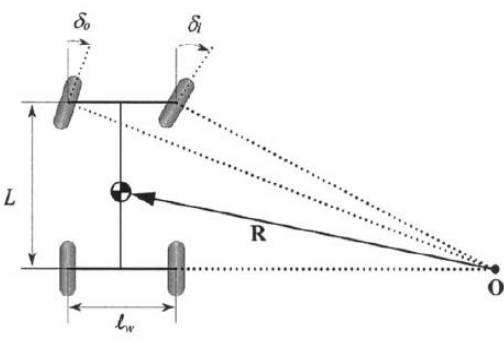
\includegraphics[width=0.5\linewidth]{figs/modelo_ackerman.png}
        \caption{Modelo cinemático de Ackerman}
        \label{fig:modelo_ackerman}
    \end{figure}

    \item El motor eléctrico se representa mediante un modelo continuo promediado. No se modelará la conmutación discreta ni el control PWM.

    \item Se asume acoplamiento exclusivamente a través del par motor. No se consideran efectos eléctricos secundarios como inductancia mutua, histéresis magnética ni corrientes parásitas.

    \item La rigidez del acoplamiento entre el motor y la carga se modela mediante un resorte lineal. No se incluyen deformaciones plásticas ni rigidez no lineal.

    \item La fricción se modela únicamente como viscosa, proporcional a la velocidad. Se omiten componentes estáticas o dependientes del régimen de operación.

    \item Se adopta un enfoque de parámetros concentrados tanto para las masas como la rigidez mecánica. No se consideran efectos distribuidos ni modos flexibles.

    \item La carga sobre la cremallera se representa como una masa puntual con fricción viscosa.

    \item Se considera un único actuador de dirección, sin modelar la relación entre ambas ruedas ni la geometría completa de la dirección del vehículo.
\end{itemize}

\subsubsection{Verificación con SimScape}
En la figura \ref{fig:simscape_vs_ss_diagrama} se ve cómo se llevó a cabo el diseño del sistema utilizando las herramientas de modelado de SimScape para utilizar de referencia y poder verificar si las ecuaciones para el sistema en espacio de estados han sido correctamente desarrolladas.

\begin{figure}[H]
    \centering
    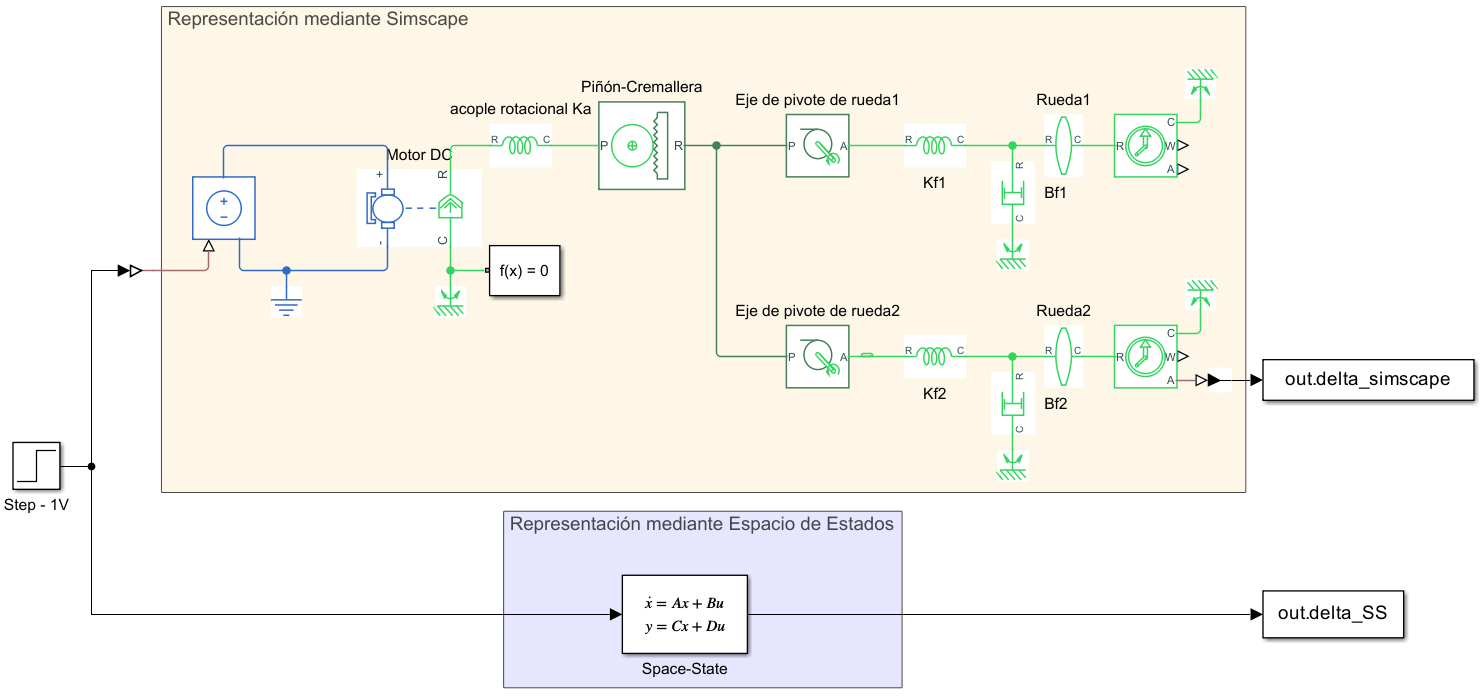
\includegraphics[width=\linewidth]{figs/simscape_SS_diagrama.png}
    \caption{Diseño del modelo en SimScape y en Espacio de Estados}
    \label{fig:simscape_vs_ss_diagrama}
\end{figure}

\begin{figure}[H]
    \centering
    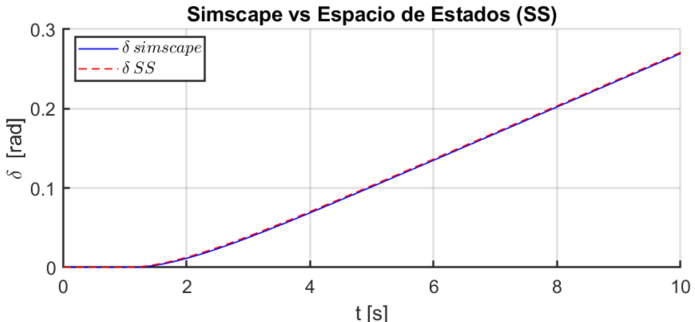
\includegraphics[width=0.75\linewidth]{figs/simscape vs SS.png}
    \caption{Variación de $\delta(t)$ con una entrada escalón $V_m = 1 \mathrm{V}$ }
    \label{fig:simscape_vs_ss}
\end{figure}

El resultado obtenido en ambos modelos es similar, y además es consistente con los resultados esperados, ya que al aplicar una entrada escalón de voltaje al motor, las ruedas deberían girar indefinidamente (sin considerar las limitaciones mecánicas en el rango de movimiento). Para este proyecto es de mayor conveniencia utilizar el sistema en espacio de estados debido a la facilidad que presenta para el diseño de controladores y observadores.

\subsubsection{Análisis de estabilidad}

Los polos de un sistema lineal expresado en espacio de estados pueden ser encontrados al calcular los autovalores de la matriz $A$, ya que estos representan la dinámica natural del sistema sin control. Se debe resolver la siguiente ecuación característica:

\begin{equation}
    \det(sI - A) = 0
\end{equation}

Al resolverlo de forma numérica en MATLAB se obtienen los siguientes polos:

\begin{table}[H]
\small
\centering
\caption{Polos del sistema de dirección por cable}
\label{tab:polos_modelo}
\begin{tabular}{c c}
\toprule
\textbf{Polo} & \textbf{Valor [$\mathrm{rad/s}$]} \\
\midrule
$p_1$ & $-0.8 + 1317.5i$ \\
$p_2$ & $-0.8 - 1317.5i$ \\
$p_3$ & $-299.9$ \\
$p_4$ & $0$ \\
$p_5$ & $-1.1$ \\
$p_6$ & $-54.8 + 276.8i$ \\
$p_7$ & $-54.8 - 276.8i$ \\
\bottomrule
\end{tabular}
\end{table}

Los polos del sistema se ubican todos en el semiplano izquierdo del plano complejo, con excepción de uno que se encuentra en el origen. Esto indica que el sistema es marginalmente estable. El polo $p_4 = 0$ corresponde a un modo integrador, lo cual se debe a una acumulación de estado sin disipación. Esto puede verse en la figura \ref{fig:simscape_vs_ss}, donde ante una entrada de tensión, el ángulo de las ruedas aumenta indefinidamente. Los polos $p_1 = -0.8 + 1317.5i$ y $p_2 = -0.8 - 1317.5i$ presentan una parte imaginaria elevada con poca atenuación, lo que refleja modos altamente oscilatorios característicos de la dinámica eléctrica del motor. Por otro lado, los polos $p_6 = -54.8 + 276.8i$ y $p_7 = -54.8 - 276.8i$ representan modos más lentos, con menor frecuencia y amortiguamiento, que dominan la respuesta visible del sistema mecánico.

\subsubsection{Análisis de controlabilidad desde la entrada \texorpdfstring{$V_m$}{}}

Un sistema en espacio de estados es completamente controlable si es posible llevar el estado desde cualquier condición inicial hasta cualquier otra en un tiempo finito mediante una entrada adecuada. Matemáticamente, la condición de controlabilidad se verifica a través del rango de la matriz de controlabilidad $\mathcal{C}$ que, para este sistema de orden 7, se define como:

\begin{equation}
\mathcal{C} = \begin{bmatrix}
B & AB & A^2B & A^3B & A^4B & A^5B & A^6B 
\end{bmatrix}
\end{equation}

Si la matriz $\mathcal{C}$ tiene rango completo, luego, el sistema es completamente controlable. Esto ocurre cuando su determinante es diferente de cero. Dicha matriz fue construida simbólicamente en MATLAB utilizando los parámetros del modelo, y calculado el determinante se obtiene la siguiente expresión:

\begin{equation}
\det(\mathcal{C}) = -\frac{K_f^2 \, K_s^4 \, K_t^6}{J_f^2 \, J_m^6 \, L_m^7 \, M_{cr}^4 \, r_L^2 \, r_P^4} = -1.9658 \times 10^{44}
\end{equation}

Esta expresión es estrictamente negativa para valores físicos positivos de los parámetros involucrados, lo cual implica que la matriz de controlabilidad es de rango completo y, por lo tanto, el sistema es completamente controlable desde la entrada de tensión del motor.

\subsubsection{Análisis de observabilidad desde la salida \texorpdfstring{$\theta_m$}{} }

Un sistema en espacio de estados es completamente observable si, a partir de la evolución temporal de la salida, es posible reconstruir todos los estados del sistema en un tiempo finito. Matemáticamente, esta propiedad se verifica a través del rango de la matriz de observabilidad $\mathcal{O}$ que, para este sistema de orden 7, se define como:

\begin{equation}
\mathcal{O} = \begin{bmatrix}
C \\
CA \\
CA^2 \\
CA^3 \\
CA^4 \\
CA^5 \\
CA^6 
\end{bmatrix}
\end{equation}

Si la matriz $\mathcal{O}$ tiene rango completo, entonces el sistema es completamente observable. En este trabajo, se consideró como salida la variable $\delta$, correspondiente al sexto estado del sistema. La matriz $\mathcal{O}$ fue construida simbólicamente en MATLAB, y el cálculo de su determinante condujo a la siguiente expresión simbólica:

\begin{equation}
\det(\mathcal{O}) = 
\frac{4\,K_f^2 \,K_s^4 \,K_t\,\Phi}{J_f\,J_m^5 \,L_m^4 \,M_{cr}^3 \,r_L^4 \,r_P^6}
\end{equation}

donde el numerador incluye el siguiente término:

\begin{align*}
\Phi =\; &K_f\,K_s\,L_m^4 \,r_L^2 + 2\,J_f\,K_f\,L_m^2 \,R_m^2 \,r_P^2 + J_f\,K_s\,L_m^2 \,R_m^2 \,r_L^2 + J_f\,M_{cr}\,R_m^4 \,r_L^2 \,r_P^2 \\
&- 2\,B_f\,K_f\,L_m^3 \,R_m\,r_P^2 - B_f\,K_s\,L_m^3 \,R_m\,r_L^2 - B_{cr}\,J_f\,L_m\,R_m^3 \,r_L^2 \,r_P^2 \\
&- B_{cr}\,K_f\,L_m^3 \,R_m\,r_L^2 \,r_P^2 - B_f\,L_m\,M_{cr}\,R_m^3 \,r_L^2 \,r_P^2 \\
&+ B_{cr}\,B_f\,L_m^2 \,R_m^2 \,r_L^2 \,r_P^2 + K_f\,L_m^2 \,M_{cr}\,R_m^2 \,r_L^2 \,r_P^2
\end{align*}

Al sustituir los valores numéricos de los parámetros físicos utilizados en el modelo, se obtiene:

\begin{equation}
\det(\mathcal{O}) = 2.6397 \times 10^{39}
\end{equation}

Este valor elevado y positivo confirma que la matriz de observabilidad es no singular y de rango completo, lo que implica que el sistema es completamente observable desde la medición de la variable $\theta_m$.

\subsection{Diseño de controlador}

Para el diseño del controlador se ha optado por la utilización del método LQR (Linear Quadratic Regulator). Este método busca minimizar la siguiente función de costo:

\begin{equation}
J \;=\; \int_{0}^{\infty}\bigl(x(t)^{T}\cdot Q_x \cdot x(t)\;+\;u(t)^{T} \cdot Q_u \cdot u(t)\bigr)\,dt
\end{equation}

La ley de control queda definida como:

\begin{equation}
u(t)\;=\;-K\,x(t)\;+\;k_{r}\,r(t)
\end{equation}

donde $K$ se obtiene resolviendo la ecuación de Riccati asociada y $k_{r}$ ajusta la ganancia de la referencia.  
Se ha preferido LQR sobre un controlador PID por su capacidad de penalizar simultáneamente desviaciones de estado y esfuerzo de control, lo que facilita limitar la saturación del actuador y garantizar un compromiso óptimo entre desempeño transitorio y magnitud de la señal de control.

Lo realmente importante de este método es definir correctamente las matrices $Q_x$ y $Q_u$. Normalmente, a $Q_x$ se la define teniendo en cuenta el límite máximo de cada variable de estado; pero en este caso, resulta más interesante limitar la corriente $i_m(t)$ y el ángulo de las ruedas delanteras $\delta(t)$. La primera penalización es útil para evitar picos elevados de corriente durante tiempos prolongados que puedan dañar al motor por sobrecalentamiento, y la segunda, es útil para limitar el exceso de desplazamientos en las ruedas, lo que haría llegar al sistema mecánico a sus límites físicos. Notar que estas son las variables seleccionadas como salidas de desempeño en la ecuación \ref{eq:salida_performance}. Para esto, se utiliza la regla de Bryson adaptable, donde se arma en primera instancia una matriz $Q_p$ que contenga los límites de estas variables seleccionadas.

\begin{equation}
Q_{p} =
\begin{bmatrix}
\alpha_{i}/i_{m-max}^2 & 0 \\
0 & \alpha_{\delta}/\delta_{max}^2\\
\end{bmatrix}
\end{equation}

Luego, se puede calcular la matriz $Q_x$ de orden 7:

\begin{equation}
Q_{x} = C_p^T \cdot Q_p \cdot C_p
\end{equation}

Además, se define $Q_u$ como:

\begin{equation}
Q_{u} = \frac{\rho}{V_{m-max}^2}
\end{equation}

Los coeficientes $\alpha_{i}$, $\alpha_{\delta}$ y $\rho$ se eligen para equilibrar el desempeño transitorio y magnitud de $u(t)$: aumentando cada $\alpha$ se incrementa la rigidez en esa variable, y aumentando $\rho$ se penaliza más el esfuerzo de control. En la tabla \ref{tab:valores_maximos_lqr} se definen los valores máximos para las variables de importancia en el control LQR.

\begin{table}[H]
\small
\centering
\caption{Valores máximos para variables de desempeño y entrada de control}
\label{tab:valores_maximos_lqr}
\begin{tabular}{c c}
\toprule
\textbf{Variable} & \textbf{Valor máximo recomendado} \\
\midrule
$i_{m-max}$ & $60 \; \mathrm{A}$ \\
$\delta_{max}$ & $0.31 \; \mathrm{rad} \; = 35^\circ$ \\
$V_{m-max}$ & $48 \; \mathrm{V}$ \\
\bottomrule
\end{tabular}
\end{table}

Una vez definidas estas matrices, puede calcularse $K$ con la función \texttt{lqr(A, Bc, Qx, Qu)} de MATLAB, y la ganancia de referencia se calcula como:

\begin{equation}
k_{r} = -\bigl(C_{p} \cdot (A - B_{c} \cdot K)^{-1} \cdot B_{c}\bigr)^{-1}
\end{equation}

A continuación se muestran unas imágenes del control LQR final, luego de probar distintos valores para los parámetros $\alpha$ y $\rho$:

%\begin{figure}[H]
%    \centering
%    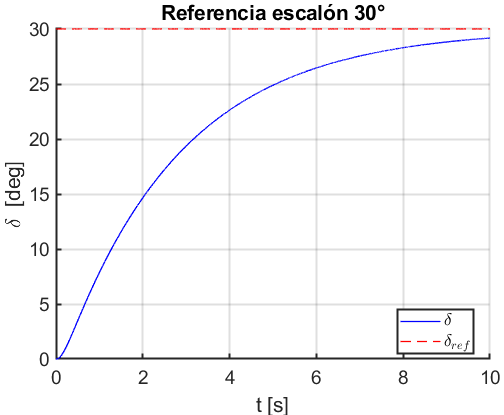
\includegraphics[width=0.7\linewidth]{figs/lqr_ref_escalon_delta_parametros_iniciales.png}
%    \caption{$\alpha_{i}=\alpha_{\delta}=\rho=1$}
%\end{figure}

\begin{figure}[H]
  \centering
  \begin{subfigure}[b]{0.48\linewidth}
    \centering
    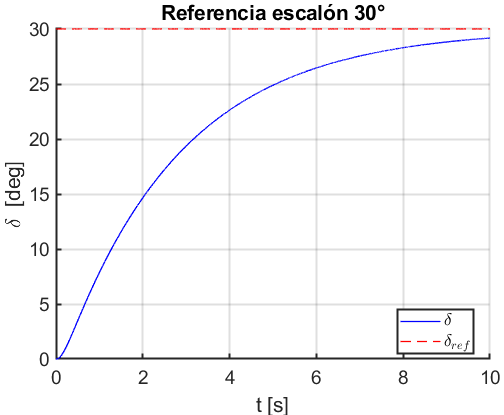
\includegraphics[width=\linewidth]{figs/lqr_ref_escalon_delta_parametros_iniciales.png}
    \caption{$\alpha_{i}=\alpha_{\delta}=\rho=1$}
    \label{fig:lqr_basico}
  \end{subfigure}
  \hfill
  \begin{subfigure}[b]{0.48\linewidth}
    \centering
    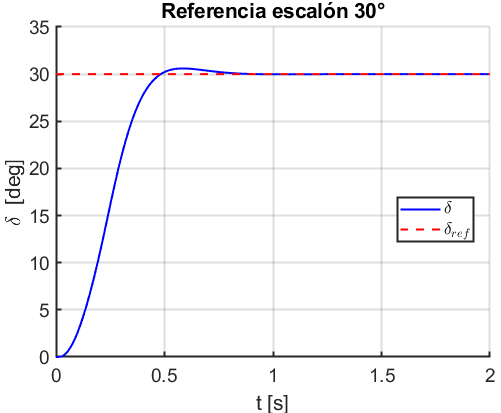
\includegraphics[width=\linewidth]{figs/lqr_ref_escalon_delta_parametros_finales.png}
    \caption{$\alpha_{i}=0.01 , \;\alpha_{\delta}=10, \;\rho=0.5$}
    \label{fig:lqr_modificado}
  \end{subfigure}
  \caption{Comparación en la respuesta al variar los parámetros}
  \label{fig:lqr_comparacion_parametros}
\end{figure}

En la figura \ref{fig:lqr_modificado} puede verse cómo al ajustar los parámetros se logra una respuesta 10 veces más rápida a la que se obtiene en \ref{fig:lqr_basico} con los parámetros en $1$.

En esta aplicación en particular, es necesario que la dirección de las ruedas responda de forma veloz a los comandos introducidos mediante el volante. El caso particular de la figura \ref{fig:lqr_comparacion_parametros} se da en una situación de estacionamiento en la que el vehículo se encuentra detenido y realiza amplias rotaciones ($>30^\circ$) de los neumáticos delanteros.

Sin embargo, al encontrarse en velocidad, entra en efecto el torque de autoalineamiento $T_a$. Este se analizará con mayor detenimiento en la sección *INSERTAR SECCION DE PERTURBACIONES*, pero por ahora será considerado como una perturbación constante. Al querer realizar un giro de $10^\circ$ en velocidad, entrará en efecto esta perturbación, lo que genera un error de estado estacionario, como puede verse en la figura \ref{fig:error_estado_estacionario}.

\begin{figure}[H]
    \centering
    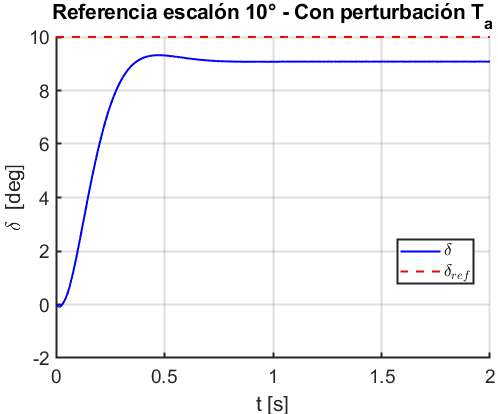
\includegraphics[width=0.5\linewidth]{figs/error_estado_estacionario.png}
    \caption{Presencia de error de estado estacionario}
    \label{fig:error_estado_estacionario}
\end{figure}

\subsubsection{Implementación propuesta de $T_a$ por rueda}

Del análisis del modelo dinámico se concluye que la variable $\delta$ representa el comportamiento de una rueda delantera representativa, mientras que la cremallera recibe el efecto conjunto de ambas ruedas mediante los términos duplicados en $K_f$. En consecuencia, resulta más consistente modelar el torque autoalineante $T_a$ \textbf{por rueda}, suponiendo que la otra rueda presenta el mismo ángulo y el mismo comportamiento.

La siguiente función de MATLAB implementa esta idea. El modelo bicicleta se utiliza para obtener el ángulo de deriva delantero $\alpha_f$, pero la fuerza lateral y el torque autoalineante se calculan para una única rueda delantera:

\begin{verbatim}
function [Ta, alpha_f, vy, r] = CalculoTaPorRueda(delta, vel_kmh)
% CalculoTaPorRueda
% Calcula el torque autoalineante por rueda delantera,
% suponiendo que ambas ruedas delanteras tienen el mismo
% angulo y comportamiento.
%
% Entradas:
%   delta    [rad]   angulo de rueda delantera
%   vel_kmh  [km/h]  velocidad vehicular
%
% Salidas:
%   Ta       [N*m]   torque autoalineante por rueda
%   alpha_f  [rad]   slip angle delantero
%   vy       [m/s]   velocidad lateral CG (steady-state)
%   r        [rad/s] yaw rate (steady-state)

    % Parametros vehiculo
    m = 1400;
    g = 9.80665;
    L = 2.70;
    a = 1.20;
    b = L - a;

    % Rigideces por eje para el modelo bicicleta
    Cf_axle = 8e4;   % [N/rad]
    Cr_axle = 8e4;   % [N/rad]

    % Parametros de saturacion / trail
    mu = 0.90;
    t0 = 0.08;       % [m]
    kAlpha = 8.0;
    Vt = 40;         % [m/s]

    Vx = vel_kmh / 3.6;

    if Vx < 0.5
        Ta = 0;
        alpha_f = 0;
        vy = 0;
        r = 0;
        return
    end

    Vx_eff = max(Vx, 0.5);

    % Modelo bicicleta en regimen estacionario
    M11 = Cf_axle + Cr_axle;
    M12 = m * Vx_eff^2 + Cf_axle * a - Cr_axle * b;

    M21 = a * Cf_axle - b * Cr_axle;
    M22 = a^2 * Cf_axle + b^2 * Cr_axle;

    rhs1 = Cf_axle * Vx_eff * delta;
    rhs2 = a * Cf_axle * Vx_eff * delta;

    M = [M11, M12; M21, M22];
    rhs = [rhs1; rhs2];

    sol = M \ rhs;
    vy = sol(1);
    r = sol(2);

    % Slip delantero comun a ambas ruedas
    alpha_f = delta - (vy + a * r) / Vx_eff;

    % Conversion a magnitudes por rueda
    Cf_wheel = Cf_axle / 2;
    Fzf_wheel = ((b / L) * m * g) / 2;
    Fy_max_wheel = mu * Fzf_wheel;

    % Fuerza lateral por rueda con saturacion suave
    Fy_lin_wheel = Cf_wheel * alpha_f;
    Fy_wheel = Fy_max_wheel * tanh(Fy_lin_wheel / Fy_max_wheel);

    % Trail efectivo
    trail = t0 * exp(-kAlpha * abs(alpha_f)) * ...
            (1 / (1 + (Vx_eff / Vt)^2));

    % Torque autoalineante por rueda
    Ta = -Fy_wheel * trail;
end
\end{verbatim}

Con esta reformulación, el torque autoalineante aplicado en la ecuación de la rueda resulta coherente con una única rueda delantera. Si ambas ruedas se comportan simétricamente, entonces la otra rueda tendrá el mismo valor de torque autoalineante.

\subsubsection{Controlador LQR con acción integral}

Para eliminar el error en estado estacionario frente a referencias constantes se introduce la variable de estado
$z(t)=\int_{0}^{t}\bigl(y_{p}(\tau)-r(\tau)\bigr)\,d\tau$,
que acumula la diferencia entre la salida de desempeño $y_{p}=C_{p}x$ y la referencia $r$. De este modo se amplía el vector de estados a
\begin{equation}
x_{\mathrm{aug}}(t)=
\begin{bmatrix}
x(t)\\
z(t)
\end{bmatrix},
\end{equation}
y las ecuaciones de estado pasan a
\begin{equation}
\dot x_{\mathrm{aug}}(t)
=
\underbrace{
\begin{bmatrix}
A & 0\\
C_{p} & 0
\end{bmatrix}
}_{A_{\mathrm{aug}}}
\!x_{\mathrm{aug}}(t)
+
\underbrace{
\begin{bmatrix}
B_{c}\\
0
\end{bmatrix}
}_{B_{\mathrm{aug}}}
\,u(t)
+
\underbrace{
\begin{bmatrix}
B_{d}\\
0
\end{bmatrix}
}_{B_{d,\mathrm{aug}}}
\,d(t)
+
\underbrace{
\begin{bmatrix}
0\\
-1
\end{bmatrix}
}_{B_{r}}
\,r(t).
\end{equation}

El controlador se diseña resolviendo la ecuación de Riccati asociada al costo
\begin{equation}
J=\int_{0}^{\infty}\bigl(x_{\mathrm{aug}}(t)^{T}Q_{x}\,x_{\mathrm{aug}}(t)
+
u(t)^{T}Q_{u}\,u(t)\bigr)\,dt.
\end{equation}
Se eligen las matrices de peso como
\begin{equation}
Q_{x}=
\begin{bmatrix}
C_{p}^{T}\,Q_{y}\,C_{p} & 0\\
0 & \displaystyle \frac{\alpha_{z}}{z_{\max}^{2}}
\end{bmatrix},
\quad
Q_{y}=\frac{\alpha_{\delta}}{\delta_{\max}^{2}},
\quad
Q_{u}=\frac{\rho}{V_{m\text{-max}}^{2}},
\end{equation}
donde $\alpha_{\delta}$ y $\alpha_{z}$ ponderan la penalización sobre $\delta$ y sobre la integral del error.

La ganancia aumentada se obtiene en MATLAB con
\begin{equation}
K_{\mathrm{aug}}=\mathrm{lqr}\bigl(A_{\mathrm{aug}},B_{\mathrm{aug}},Q_{x},Q_{u}\bigr).
\end{equation}
De $K_{\mathrm{aug}}=[\,K\;\;K_{i}\,]$ se extraen directamente
\begin{equation}
K\in\mathbb{R}^{1\times 7},
\quad
K_{i}\in\mathbb{R},
\end{equation}
que se emplean en la ley de control
\begin{equation}
u(t)=-K\cdot x(t)-K_{i}\cdot z(t)
\end{equation}

Notar que la referencia ha sido quitada de la ley de control ya que se encuentra implícita dentro de la variable de estado $z(t)$.


\subsection*{Fuentes utilizadas para el modelado del torque autoalineante $T_a$}

Para revisar el orden de magnitud y la forma funcional del torque autoalineante se utilizaron las siguientes fuentes externas:

\begin{itemize}
    \item \textbf{Georg Rill, \textit{First Order Tire Dynamics}}. Disponible en: \url{https://www.researchgate.net/publication/317036997_First_Order_Tire_Dynamics}. De esta fuente se tomó la relación física básica entre torque autoalineante y fuerza lateral, expresada como $T_S = c_o F_y$, donde $c_o$ representa el \textit{pneumatic trail}. Esta idea se utilizó como base para escribir $T_a$ como producto entre fuerza lateral y brazo efectivo del neumático, con signo restaurador.

    \item \textbf{ScienceDirect Topics, \textit{Aligning Torque}}. Disponible en: \url{https://www.sciencedirect.com/topics/engineering/aligning-torque}. De esta fuente se extrajo el comportamiento cualitativo esperado del torque autoalineante en neumáticos reales: crecimiento aproximadamente lineal para ángulos de deriva pequeños, aparición de un máximo a bajos ángulos de deriva y disminución posterior al aumentar el deslizamiento lateral. También se utilizó para justificar que el \textit{pneumatic trail} disminuye cuando crece el ángulo de deriva.

    \item \textbf{ScienceDirect Topics, \textit{Brush Model}}. Disponible en: \url{https://www.sciencedirect.com/topics/engineering/brush-model}. De esta fuente se tomó la interpretación mecánica del origen del torque autoalineante mediante la distribución no simétrica de esfuerzos en la huella de contacto, y la observación de que un valor más realista del \textit{trail} a bajo deslizamiento puede aproximarse como $t \approx 0.5\,a$, siendo $a$ la semilongitud de la huella. Este criterio se utilizó como referencia para contrastar el valor de \textit{trail} adoptado en el modelo simplificado.

    \item \textbf{Turan Alp Arslan et al., \textit{Investigation of the Effects of Axle Load on Tyre Behaviour in Vehicles}}. Disponible en: \url{https://www.researchgate.net/publication/365781200_Investigation_of_the_Effects_of_Axle_Load_on_Tyre_Behaviour_in_Vehicles}. De este trabajo se tomaron supuestos geométricos y de carga para un neumático individual 205/55R16, en particular el uso de una muestra de una sola rueda, la presión de inflado del orden de $220.632\ \mathrm{kPa}$ y la relación entre ancho efectivo de huella y ancho del neumático. Estos datos se usaron en el análisis en Python para estimar una longitud de huella razonable por rueda y, a partir de ella, un orden de magnitud plausible del \textit{pneumatic trail}.

    \item \textbf{Hsu, Laws y Gerdes, \textit{Estimation of Tire Slip Angle and Friction Limits Using Steering Torque}}. Disponible en: \url{https://www.researchgate.net/publication/224603533_Estimation_of_Tire_Slip_Angle_and_Friction_Limits_Using_Steering_Torque}. De esta referencia se utilizó la idea de que la información del torque de dirección está fuertemente vinculada con la evolución del \textit{pneumatic trail}, y que la caída de dicho \textit{trail} es un indicador físicamente consistente del acercamiento a la saturación lateral del neumático.
\end{itemize}

En conjunto, estas fuentes se utilizaron para justificar que el análisis del torque autoalineante debía realizarse \textbf{por rueda}, suponiendo comportamiento simétrico de ambas ruedas delanteras, y que el modelo debía preservar tanto la dependencia con la fuerza lateral como la disminución del \textit{trail} a medida que aumenta el ángulo de deriva.



\end{document}
